
\documentclass[a4paper,14pt,oneside,pdflatex,english,final,twocolumn]{article}

\usepackage[utf8]{inputenc}
\usepackage{parallel}
\usepackage{siunitx}
\usepackage{booktabs}
\usepackage{fancyhdr}
\usepackage{pdfpages} 

\usepackage[export]{adjustbox}
\usepackage[margin=0.5in]{geometry}
\addtolength{\topmargin}{0in}

\usepackage{libertine}
\renewcommand*\familydefault{\sfdefault}  %% Only if the base font of the document is to be sans serif
\usepackage[T1]{fontenc}

\setlength{\parindent}{4em}
\setlength{\parskip}{1em}
\renewcommand{\baselinestretch}{1.0}

\title{ATX Power Supply splitter for Raspberry Pi Clusters}
\author{semaf}
\date{August 2020}

\begin{document}

\pagestyle{fancy}

\lhead{Semaf Electronics}
\chead {\today}
%%\rhead{bune3}

\onecolumn

\begin{figure}[ht]
	%%\begin{minipage}{0.47\textwidth}
	%%	\centering
	%%	
\includegraphics[width=.7\textwidth,left,]{img/semaf_logo.png}
	%%\end{minipage}
	%%\hfill
	\begin{minipage}{1.0\textwidth}
		\raggedleft
		\Huge \textbf{ATX Power Supply splitter for} \\
		\Huge \textbf{Raspberry Pi Clusters}
	\end{minipage}

	\vspace{1cm}
	\begin{minipage}{0.47\textwidth}

		\section{Overview}
		\begin{itemize}
			\item 8x USB-A port for 5V output
			\item Voltage, Current and power measurements
			\item 2x 5V output for general purposes
			\item 2x 12V output for general purposes
			\item 2x FAN connector
		\end{itemize}


	\end{minipage}
	\hfill
	\begin{minipage}{0.47\textwidth}
		\centering
		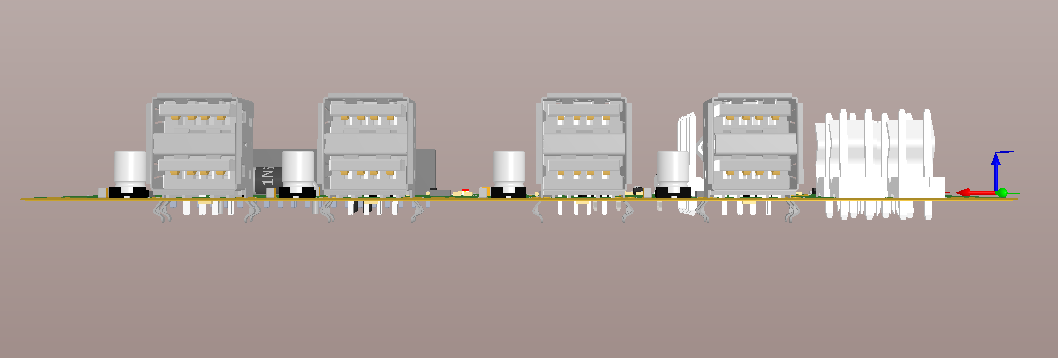
\includegraphics[width=1.0\textwidth,right]{img/Alt_USB.png}

	\end{minipage} \\
	\vspace{1cm}

	\begin{minipage}{1\textwidth}
		\section{Description}
		\par
		The ATX power splitter utilizes ATX power to split the power to 8x USB port for Raspberry Pi cluster applications. Raspberry Pi Zero can be used to control the board and read voltage and current measurements by plugging it to 40-pin header connector. Voltage, current and power measurement for each channel are available on I²C bus. Raspberry Pi Zero is powered by 5V Standby current from ATX power supply. 
		\par There are 2 connctors for standard 4-pin FAN and they can be controlled by Raspberry Pi with PWM output. FAN RPMs are also available for Reaspberry Pi to read. One user button and one user LED are available for user programming. Button can be programmed as on/off switch for ATX power supply. 
		\par
		2x PAC1934 voltage and current sensors from microchip are utilized for voltage and current measurement for each channel and values are read over I²C bus by Pi Zero. Linux kernel driver and device tree blob for current sensor are available. Device I²C addresses: 0x10, 0x1F.
		\par
		If needed, An Ethernet over SPI module can be connected to 12-pin header to bring the ethernet functionality to Raspberry Pi.
		\par 
		Onboard EEPROM for board specific data as well as for HAT (Hardware Attached on Top) specifications.
		There is a 10-pin header for UART, I²C, SPI connections.
	\end{minipage}

	\vspace{1cm}
	\begin{minipage}{0.47\textwidth}
		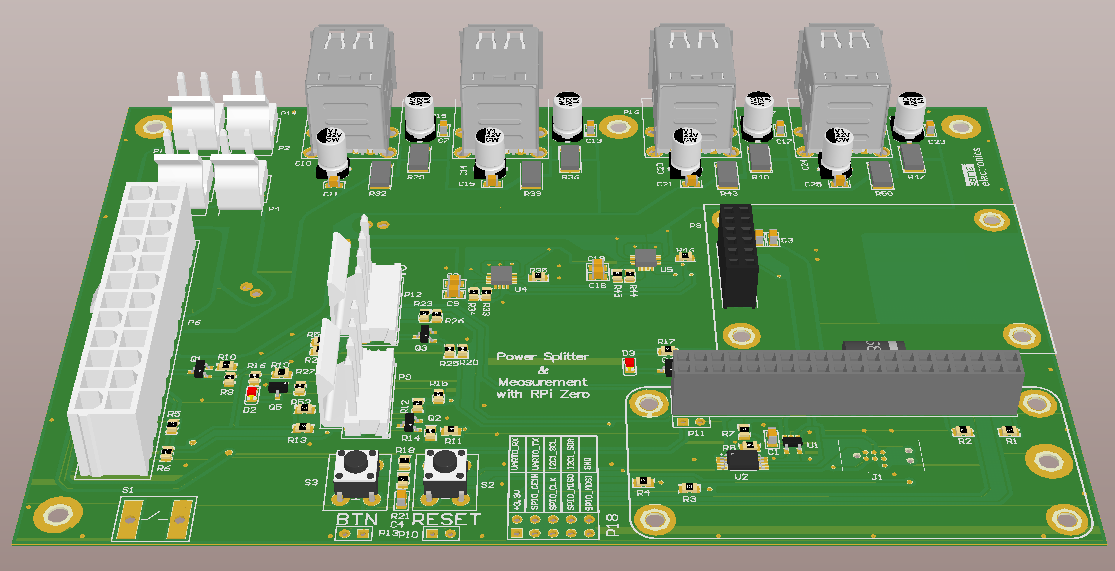
\includegraphics[width=1.0\textwidth,right]{img/Alt_Front.png}
	\end{minipage}
	\hfill
	\begin{minipage}{0.47\textwidth}
		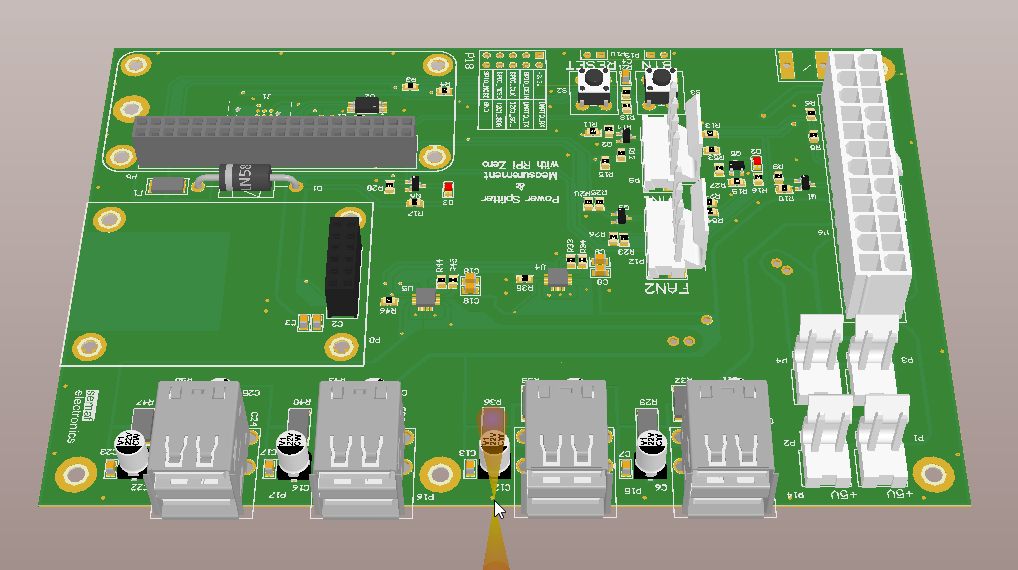
\includegraphics[width=1.0\textwidth,right]{img/Alt_Back.png}

	\end{minipage}
\end{figure}
\section{Technical specification}
\noindent
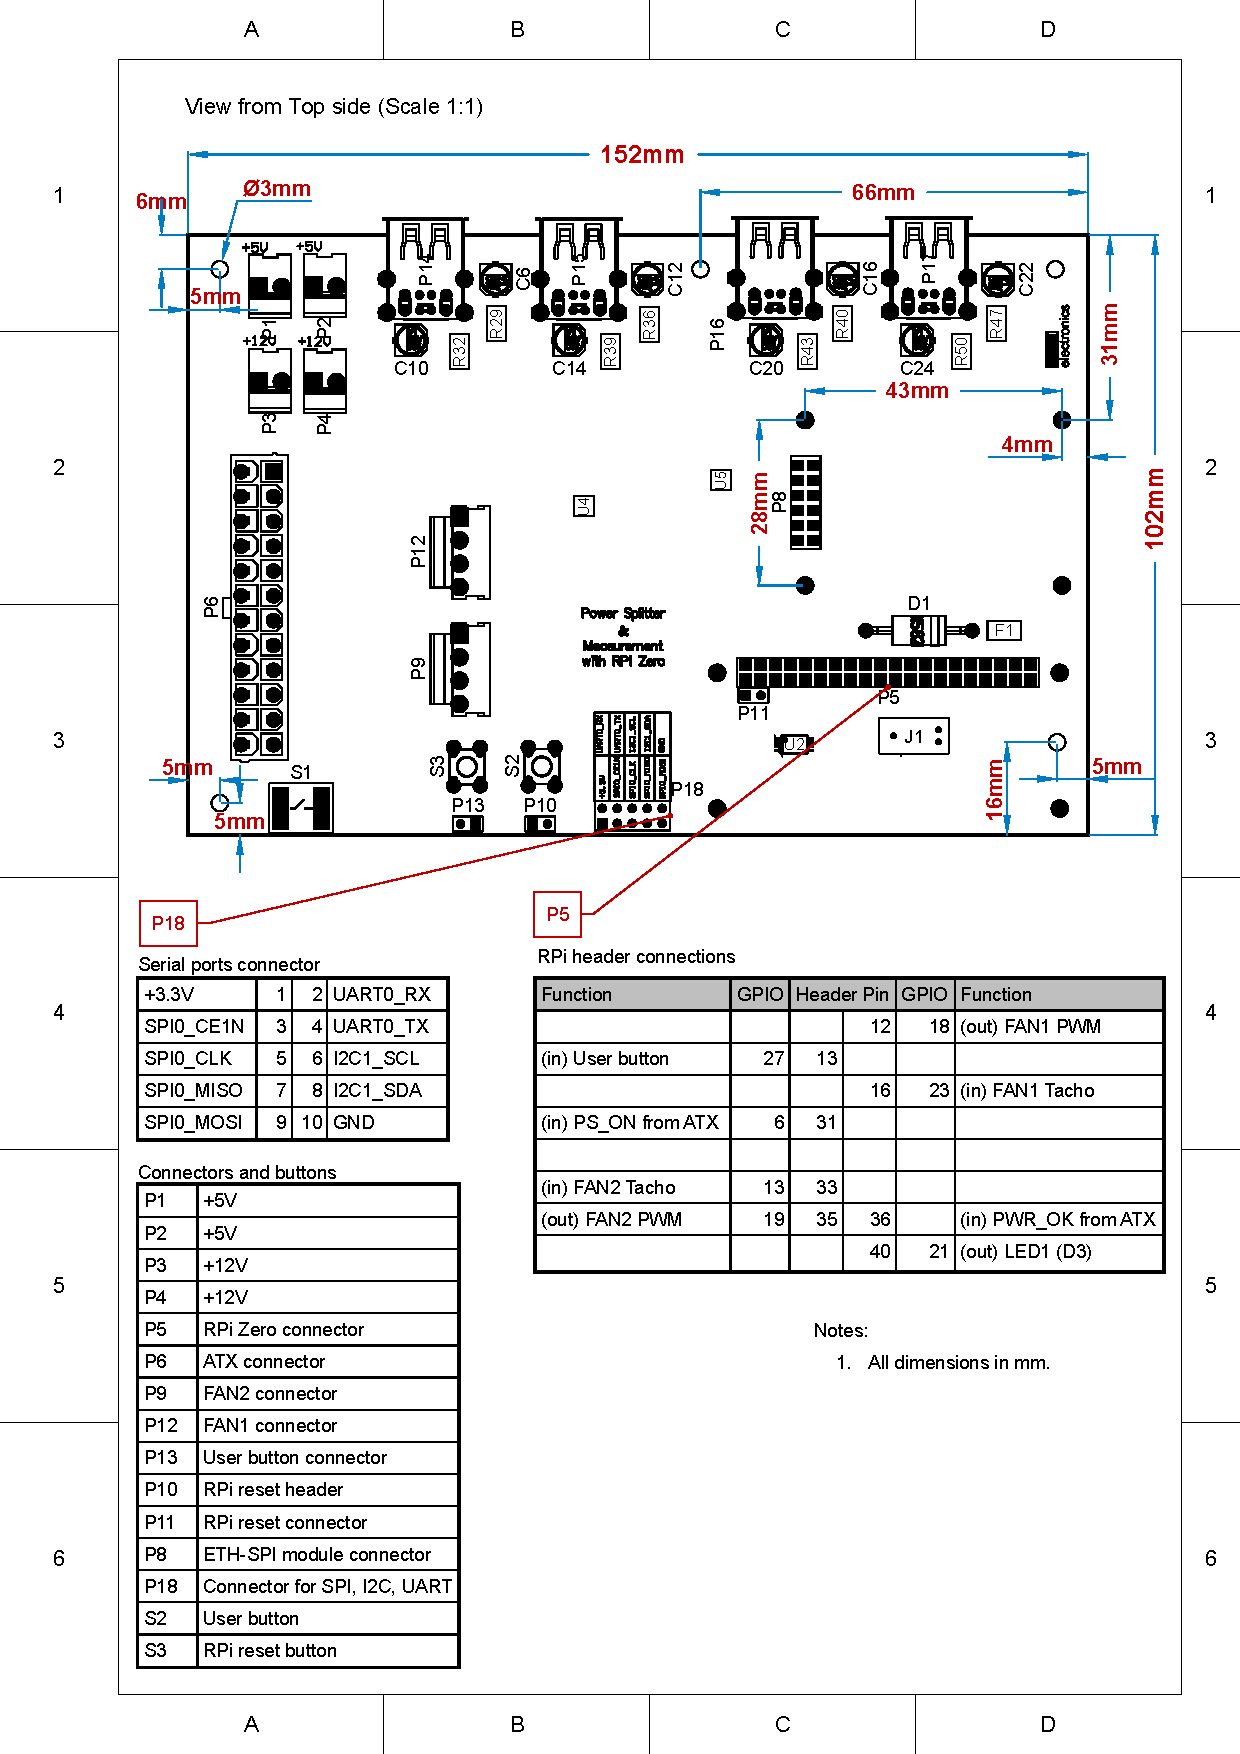
\includegraphics[
	width=\textwidth,
	height=\textheight,
	keepaspectratio
]{Drawing.pdf}
\vfill
\end{document}




